\section{Introduction}

\itbf{Goal}:

"Developing model-based non-intrusive diagnostics for SCR-ASC that can work with commercial NO-x sensors and demonstrate the results on a real-world on-road truck data."

\bigskip

\itbf{Kaushal's work}:
\begin{itemize}
    \item Diagonstic-oriented aging models for SCR-ASC.
    \begin{itemize}
        \item Chemical Kinetics based model for SCR
        \item Non-linear look-up table for ASC
    \end{itemize}
    \item Term-by-term observer design for SCR Ammonia adsorption.
    \item Diagnosis algorithm
    \begin{itemize}
        \item Sequence of filters
        \item Residual generation for fault detection using the stochastic version of the models.
    \end{itemize}
\end{itemize}

\itbf{Available measurements}
\begin{enumerate}
    \item Engine Torque
    \item Engine Speed
    \item Diesel exhaust fluid (DEF) injection
    \item Engine-out $NO_x$.
    \item Diesel oxidation catalyst (DOC)-out $NO_x$.
    \item Tail-pipe $NO_x$. (Test cell: $NH_3$ and $N_2O$)
    \item DOC-in, DOC-out, SCR-in, SCR-out and ASC-out temperatures.
    \item Exhaust flow rate.
\end{enumerate}

\itbf{Available data}
\begin{enumerate}
    \item Road data
    \begin{itemize}
        \item Cold FTP (Federal Test Procedure)
        \item Hot FTP
        \item RMC (Ramped mode cycle)
    \end{itemize}
    \item Test Cell data
    \begin{itemize}
        \item Cold FTP (Federal Test Procedure)
        \item Hot FTP
        \item RMC (Ramped mode cycle)
    \end{itemize}

\end{enumerate}

\subsection{System Setup}
\begin{figure}[H]
    \centering
    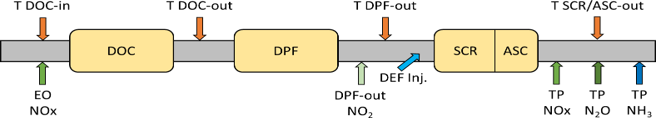
\includegraphics[width = \textwidth]{./figs/scr_system.png}
    \caption{SCR System}
\end{figure}

\subsection{Test Cell data}
From the test-cell sampling, we have
\begin{align*}
    \text{Samling time, } \qquad dt &= 0.2 \, s\\
    \text{Sampling frequency, } \quad f &= 5\, Hz
\end{align*}


\subsubsection{Test Cell data Variables}
\begin{table}[H]
\centering
\begin{tabular}{l l l c}
   \hline \hline
   Variable Name                 & Units  & Description & Variable from Model \\ \hline \hline
   LOG\_TM	                     & sec    & Time
                                          & $t$\\
   ENG\_SPD	                     & RPM    & Engine Speed
                                          &\\
   NET\_TORQ	                 & lb\_ft & Engine Torque
                                          &\\
   TEST\_CELL\_T	             & deg\_f & Test Cell Temperature
                                          &\\
   TUR\_OT\_T	                 & deg\_f & Turbine Outlet Gas Temperature
                                          &\\
   EXHAUST\_FLOW	             & kg/min & Exhaust Flow Rate
                                          & $F$\\
   V\_AIM\_TRC\_DOC\_IN	         & Deg\_C & DOC In Gas Temperature
                                          &\\
   V\_AIM\_TRC\_DOC\_OUT	     & Deg\_C & DOC Out Gas Temperature
                                          &\\
   V\_AIM\_TRC\_DPF\_OUT	     & Deg\_C & DPF Out Gas Temperature
                                          &\\
   V\_AIM\_TRC\_SCR\_OUT	     & Deg\_C & SCR/ASC Out Gas Temperature
                                          &\\
   V\_SCR\_ANR\_FDBK	         & None   & ANR (??)
                                          &\\
   V\_UIM\_FLM\_ESTUREAINJRATE	 & ml/sec & DEF (Urea Sol.) Dosing Rate
                                          & $u_2$\\
   ENG\_CW\_NOX\_FTIR\_COR\_U2	 & PPM    & Engine-Out NOx
                                          & $u_1$\\
   EXH\_CW\_NOX\_COR\_U1	     & PPM    & Tailpipe NOx
                                          & $x_1$\\
   EXH\_CW\_AMMONIA\_MEA	     & ppm    & Tailpipe NH3
                                          & $x_2$\\
   EXH\_CW\_N2O\_MEA	         & ppm    & Tailpipe N2O
                                          &\\
   ENG\_CW\_NO2\_COR\_U2	     & PPM    & DPF Outlet NO2
                                          &\\
EONOX\_COMP\_VALUE	         & ppm    & Engine-out NOx (with Corss-sensitivity)
                                      & $y_3$\\
V\_SCM\_PPM\_SCR\_OUT\_NOX	 & ppm    & SCR-out NOx  (with cross-sensitivity)                    & $y_1$\\
   \hline \hline
\end{tabular}
\caption{Test Cell Data Variables}
\end{table}

% ============================================================================
\subsubsection{Test cell data ranges}
\begin{table}[H]
\centering
\begin{tabular}{c c c c c}
\hline \hline
Variable & Units &Cold FTP & Hot FTP & RMC\\
\hline \hline
& & Degreend Data & & \\ \hline
$T$   & $^0$C & & &
\\
$F$   & $kg/min$ & & &
\\
$x_1$ & $ppm$ & & &
\\
$x_2$ & $ppm$ & & &
\\
$u_1$ & $ppm$ & & &
\\
$u_2$ & $ppm$ & & &
\\
$y_1$ & $ppm$ & & &
\\
$y_3$ & $ppm$ & & &
\\
\hline
& & Aged Data & & \\ \hline
$T$   & $^0$C & & &
\\
$F$   & $kg/min$ & & &
\\
$x_1$ & $ppm$ & & &
\\
$x_2$ & $ppm$ & & &
\\
$u_1$ & $ppm$ & & &
\\
$u_2$ & $ppm$ & & &
\\
$y_1$ & $ppm$ & & &
\\
$y_3$ & $ppm$ & & &
\\
\hline \hline
\end{tabular}
\caption{Test cell data ranges}
\end{table}


% =============================================================================

%Expt. & $F\,(kg/min)$ & $T\, (^0 C)$ & $x_1$ (ppm) & $u_1$ (ppm) & $x_2$ (ppm)
%& $u_2$ & $y_1$ & $y_3$
%\\\hline \hline
%%=======================================================================
%Aged (Cold FTP) & [0 26.64] & [28.20 262.30] & [0 558.06] & [-2.78
%760.55] & [-0.60 1.40] \\
%%=======================================================================
%Aged (Hot FTP) & [0 26.50] & [134.30 269] & [0 506.48] & [-14.40
%158.67] & [-0.60 11.10]\\
%%=======================================================================
%Aged (RMC) & [1.80 24.75] & [238.40 348.20] & [0 693.65] & [-2.24
%109.63] & [0.80 4.40]\\
%%=======================================================================
%De-greened (Cold FTP) & [0 26.72] & [25.80 253.90] & [0 609.84] &
%[-116.93 518.05] & [-0.70 1.70] \\
%%=======================================================================
%De-greened (Hot FTP) & [0 26.47] & [110.10 261.80] & [0 504.92] &
%[-17.16 110.85] & [-0.50 3.70]\\
%%=======================================================================
%De-greened (RMC) & [1.84 24.91] & [236.20 341.30] & [0 728.04] &
%[-1.30 75.61] & [0.40 5.20] \\
%

\subsection{Road data}
From the test-cell sampling, we have
\begin{align*}
    \text{Samling time, } \qquad dt &= 1 \, s\\
    \text{Sampling frequency, } \quad f &= 1 \, Hz
\end{align*}



\subsubsection{Road data variables}
\begin{table}[H]
\centering
\begin{tabular}{l l l }
\hline \hline
Model Variable & Road Data Variable &Units\\
\hline \hline
$t$   & tod & $s$
\\
$T$   & pSCRBedTemp & $^0$C
\\
$F$   & pExhMF & $kg/min$
\\
$x_1$ & & $ppm$
\\
$x_2$ & & $ppm$
\\
$u_1$ & & $ppm$
\\
$u_2$ & pUreaDosing & $ml/sec$
\\
$y_1 $ & pNOxOutppm & $ppm$
\\
$y_3 (=u_1?)$ & pNOxInppm & $ppm$
\\
\hline
\end{tabular}
\caption{Road data variables}
\end{table}


\subsubsection{Road data ranges}
\begin{table}[H]
\centering
\begin{tabular}{l l l l l l l l l l }
\hline \hline
Variable & Units & adt\_15 &adt\_17&mes\_15&mes\_18&wer\_15&wer\_20&trw\_15&trw\_16
\\
\hline \hline
$T$   & $^0$C & & & &&&&&
\\
$F$   & $kg/min$ & & & &&&&&
\\
$x_1$ & $ppm$ & & & &&&&&
\\
$x_2$ & $ppm$ & & & &&&&&
\\
$u_1$ & $ppm$ & & & &&&&&
\\
$u_2$ & $ppm$ & & & &&&&&
\\
$y_1$ & $ppm$ & & & &&&&&
\\
$y_3$ & $ppm$ & & & &&&&&
\\
\hline \hline
\end{tabular}
\caption{Road data ranges}
\end{table}


\subsection{Approach to the research problem}
Our approach is based on the presumption that the aging detection problem can be framed as a state/parameter estimation challenge with respect to the concentration dynamics of the gases involved. This gives rise to the following sub-problems:

\begin{enumerate}
\item Determining a suitable model for the system dynamics.
\item Assessing whether the available data contains sufficient information for identifying the model parameters related to the chosen system dynamics.
\item Investigating the relationship between the parameters/states and the aging factor of the catalyst.
\item Understanding the uncertainties inherent in the aforementioned processes.
\item Finally, developing and validating the aging detection algorithm.
\end{enumerate}
